\documentclass[12pt, a4paper]{report}
\usepackage[utf8]{inputenc} % Eingabekodierung
\usepackage[T1]{fontenc} % Fontkodierung
\usepackage[english]{babel} % Deutsche Sprache
\usepackage{graphicx} % Grafiken
\usepackage{hyperref} % Hyperlinks
\usepackage{geometry} % Seitenlayout
\usepackage{setspace} % Zeilenabstand
\usepackage{fancyhdr} % Kopf- und Fußzeile
\usepackage{titlesec} % Kapitelnummerierung
\usepackage{adjustbox} % Bildbearbeitung
\usepackage{subcaption}
\usepackage{titletoc}
\usepackage[backend=biber, style=authoryear, maxcitenames=1, mincitenames=1]{biblatex}
\addbibresource{2023_11_29_Seminararbeit.bib}

\geometry{a4paper, margin=2.5cm} % Seitenränder
\hypersetup{colorlinks=true, urlcolor=blue, linkcolor=black, citecolor=black} % Hyperlinks einrichten
\onehalfspacing % Zeilenabstand auf 1,5-fach setzen

\usepackage{enumitem} % Formatierung Aufzählungsverzeichnis enumerate

\makeatletter
\renewcommand{\@roman}[1]{\expandafter\@slowromancap\romannumeral #1@}
\makeatother

\usepackage[printonlyused]{acronym}

\usepackage{glossaries}
\newglossaryentry{symb:A}{
	name={\(A\)},
	description={Beschreibung des Symbols \(A\)}
}
\newglossaryentry{symb:B}{
	name={\(B\)},
	description={Beschreibung des Symbols \(B\)}
}
\makeglossaries

\pagestyle{fancy}
\fancyhf{} % Löscht alle voreingestellten Kopf- und Fußzeileneinstellungen

% Definiere die Kopfzeile
\lhead{\leftmark} % Aktuelles Kapitel auf der linken Seite
\chead{} % Kein Inhalt in der Mitte der Kopfzeile
\rhead{} % Kein Inhalt auf der rechten Seite der Kopfzeile

% Definiere die Fußzeile (optional)
\lfoot{} % Kein Inhalt auf der linken Seite der Fußzeile
\cfoot{\thepage} % Seitenzahl in der Mitte der Fußzeile
\rfoot{} % Kein Inhalt auf der rechten Seite der Fußzeile

\DeclareNameAlias{sortname}{last-first}
\renewcommand*{\nameyeardelim}{\addcomma\addspace}

%Formatierung für Online-Zitate
\DeclareCiteCommand{\citeonline}[\mkbibparens]
{\usebibmacro{prenote}}
{\usebibmacro{citeindex}%
	\printtext[bibhyperref]{%
		\printfield{title}%
		\setunit{\addcomma\space}%
		\printfield{year}}}
{\multicitedelim}
{\usebibmacro{postnote}}

\titleformat{\chapter}[hang]
{\normalfont\huge\bfseries}{\thechapter.}{0.5em}{\huge\bfseries}

\renewcommand{\figurename}{Figure}

\begin{document}

\begin{titlepage}
	\centering
	
\includegraphics[width=0.5\textwidth]{2023_11_29_Bilder_Dokumentation/hhn-logo.png}

	\vspace*{15mm}

	{\LARGE \textbf{Faculty of Engineering (TE)\\Automotive Systems Engineering}}

	\vspace*{15mm}

	{\Huge Project for Digital Signal Processing}

	\vspace*{15mm}

	{\Large Project Documentation}\\
	Master Automotive Systems Engineering\\

	by\\

	{\Large Jakob Kurz \& Mattis Tom Ritter}\\
	(Matriculation-Nr. 210262 \& 210265)\\

	\vspace{5mm}

	presented in Wintersemester 2024/25 at\\

	\vspace{5mm}

	{\Large Heilbronn University}

	\vspace*{10mm}

	\begin{tabbing}
		\hspace*{4cm}Reviewer: \hspace*{1cm}\=Prof. Dr. Volker Stahl\\
		\hspace*{4cm}Levy: \>31. December 2024
	\end{tabbing}
\end{titlepage}


\pagenumbering{gobble} % Ausschalten der Seitennummerierung

\renewcommand{\contentsname}{Table of Contents}
\tableofcontents % Inhaltsverzeichnis erstellen
\newpage

\pagenumbering{roman} % Verzeichnisse werden in römischen zahlen nummeriert´

\chapter*{List of Abbreviations}
\label{sec:abkuerzungsverzeichnis}
\begin{acronym}[OpenCV]
	\acro{DFT}{Discrete Fourier Transform}
	\acro{FFT}{Fast Fourier Transform}
\end{acronym}
\newpage

\renewcommand{\listfigurename}{List of Figures}
\listoffigures
\newpage

%\listoftables
%\newpage

%\subsection*{Symbolverzeichnis}
%\label{sec:symbolverzeichnis}
%\printglossary
%\newpage

\pagenumbering{arabic}
\setcounter{page}{1}	% Setze Seitenzähler auf 1

\chapter{Basic Implementations}

\section{\ac{DFT} vs. \ac{FFT}}

\subsection{Implementation Overview}
The \ac{DFT} and \ac{FFT} implementations are provided in \texttt{dft.py} and \texttt{fft.py}, respectively:
\begin{itemize}
	\item \textbf{\ac{DFT}}: Computes the Fourier Transform with \(O(N^2)\) complexity using a direct summation formula.
	\item \textbf{\ac{FFT}}:
	      \begin{itemize}
		      \item \textbf{Recursive FFT}: Implements a divide-and-conquer approach, reducing complexity to \(O(N \log N)\).
		      \item \textbf{Iterative FFT}: Uses iterative butterfly operations for further optimization, avoiding recursion overhead.
	      \end{itemize}
\end{itemize}

\subsection{Verification of Similarities}
The Python script \texttt{test\_dft\_fft.py} validates the numerical equivalence of the \ac{DFT} and \ac{FFT} implementations:
\begin{itemize}
	\item A sinusoidal test signal is processed by all three methods (\ac{DFT}, recursive \ac{FFT}, and iterative \ac{FFT}).
	\item Results are compared element-wise within a tolerance of \(10^{-9}\).
	\item Tests confirm that all implementations produce consistent outputs, differing only by negligible numerical errors.
\end{itemize}
\noindent The visualization script \texttt{vis\_dft\_fft\_simmiliar.py} further illustrates the similarities:
\begin{itemize}
	\item \textbf{Frequency Domain Comparison (Fig. \ref{fig:frequency_domain_comparison} Left)}: All methods accurately identify the signal's frequency components.
	\item \textbf{Time Domain Reconstruction (Fig. \ref{fig:frequency_domain_comparison} Right)}: All methods reconstruct the original signal with minimal deviations.
\end{itemize}

\begin{figure}[h!]
	\centering
	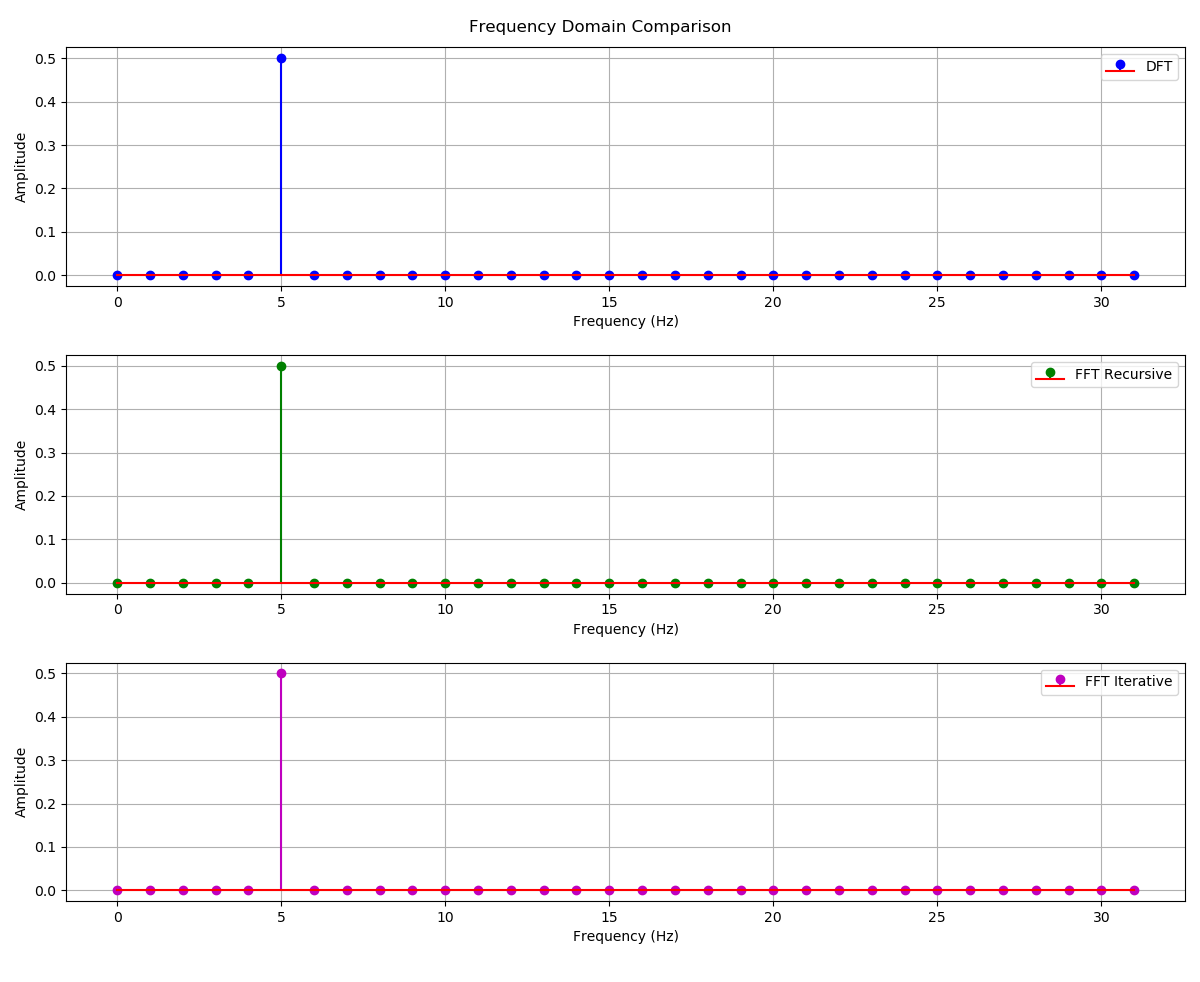
\includegraphics[width=0.45\textwidth]{2023_11_29_Bilder_Dokumentation/Frequency_Domain_Comparison.png}
	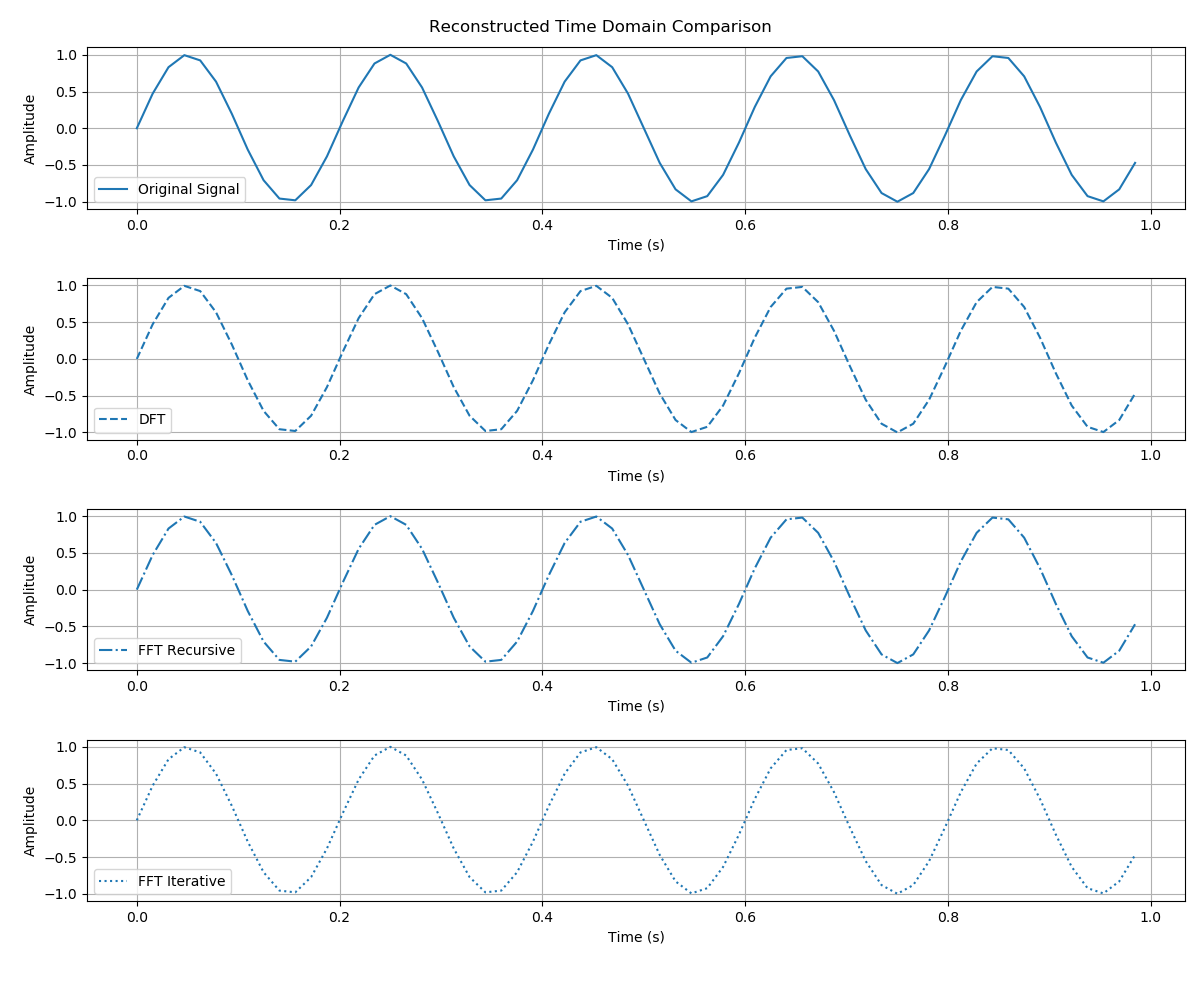
\includegraphics[width=0.45\textwidth]{2023_11_29_Bilder_Dokumentation/Time_Domain_Comparison.png}
	\caption{Frequency domain comparison (left) and Time-domain reconstruction validation (right)}
	\label{fig:frequency_domain_comparison}
\end{figure}

\subsection{Comparison of Differences}
To highlight differences, the script \texttt{vis\_dft\_fft\_different.py} visualizes computational time and memory usage for the \ac{DFT} and \ac{FFT}.

\subsubsection{Computational Time and Memory Comparison}
Figure \ref{fig:time_memory_comparison} shows the execution time and memory usage for a fixed signal length:
\begin{itemize}
	\item The \ac{DFT} requires significantly more time due to its \(O(N^2)\) complexity, while both \ac{FFT} implementations achieve \(O(N \log N)\).
	\item The iterative \ac{FFT} is slightly faster than the recursive \ac{FFT}.
	\item Memory usage for the \ac{FFT} is lower than the \ac{DFT}, with the iterative \ac{FFT} requiring the least memory.
\end{itemize}

\begin{figure}[h!]
	\centering
	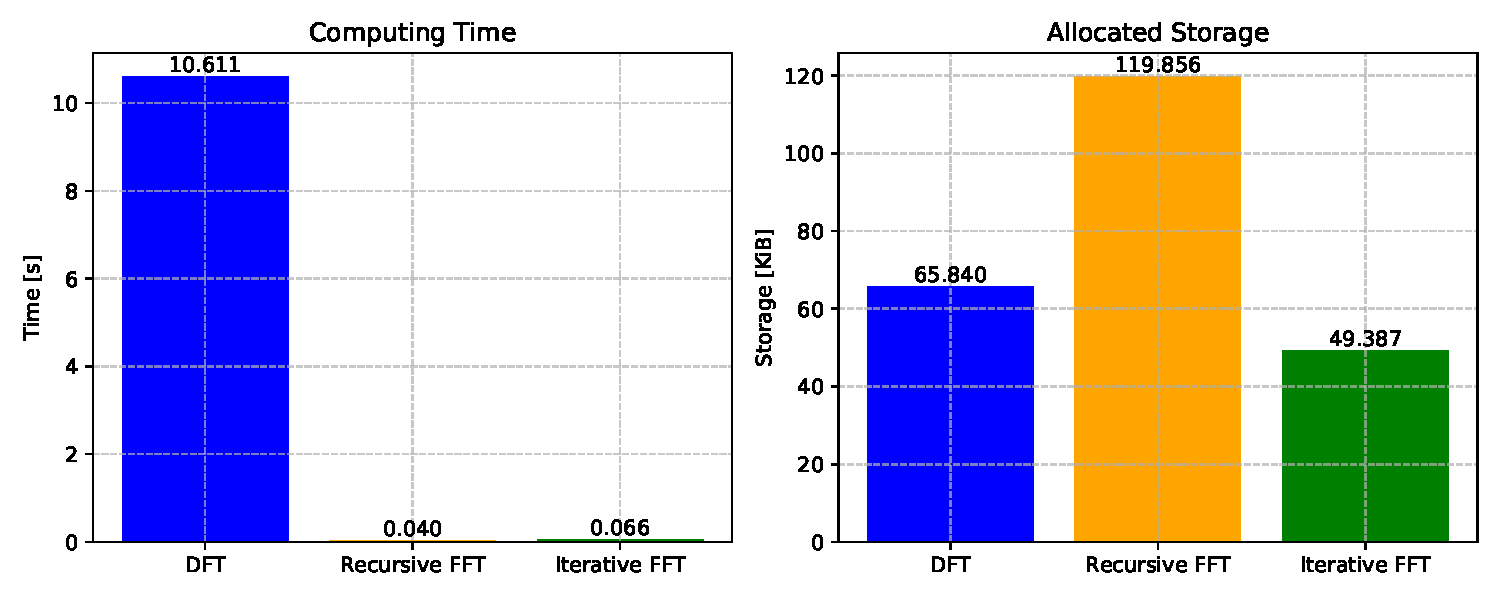
\includegraphics[width=0.9\textwidth]{figures/dft_fftr_ffti.pdf}
	\caption{Computational time for fixed signal length (left). Memory usage comparison (right).}
	\label{fig:time_memory_comparison}
\end{figure}

\subsubsection{Scaling with Signal Length}
Figure \ref{fig:scaling_comparison} examines execution time and memory usage as signal length increases:
\begin{itemize}
	\item Execution time for the \ac{DFT} grows quadratically, while the \ac{FFT} scales logarithmically.
	\item Memory usage for the \ac{DFT} increases linearly, whereas both \ac{FFT} methods maintain near-constant memory requirements.
	\item The iterative \ac{FFT} consistently outperforms the recursive \ac{FFT} in both time and memory usage.
\end{itemize}

\begin{figure}[h!]
	\centering
	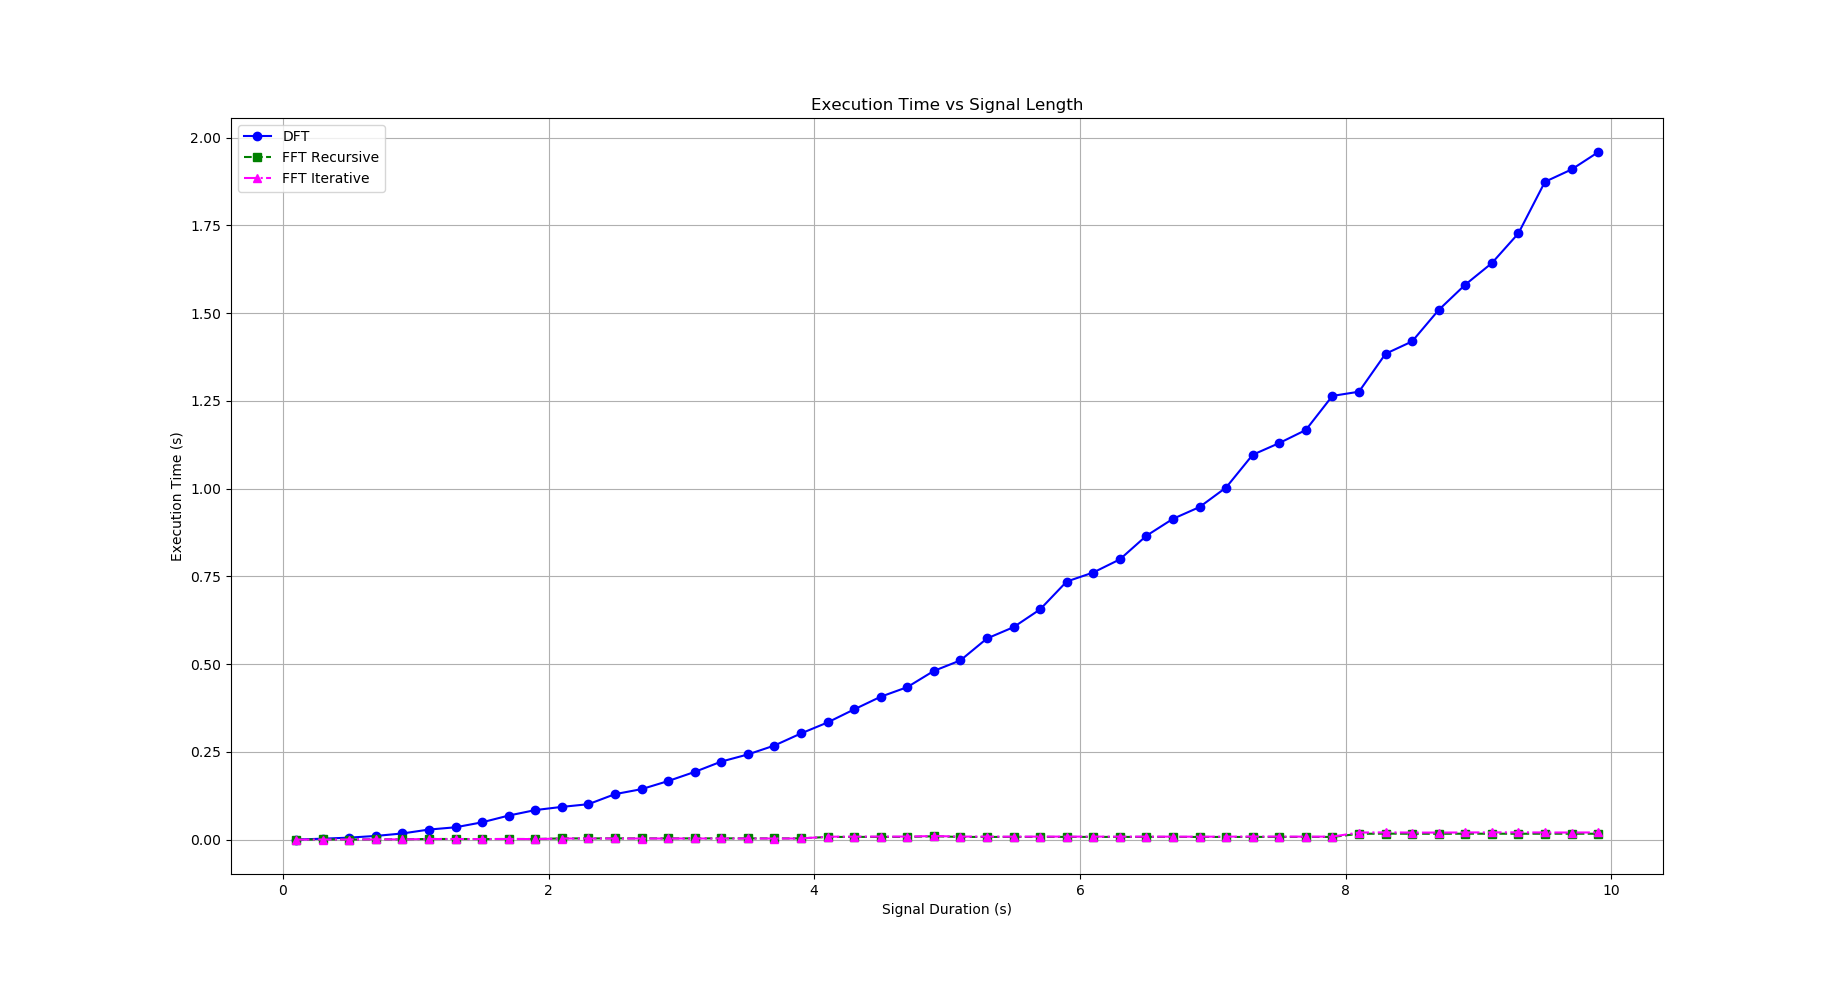
\includegraphics[width=0.45\textwidth]{2023_11_29_Bilder_Dokumentation/Execution_Time_vs_Signal_Length.png}
	\hspace{0.05\textwidth}
	\includegraphics[width=0.45\textwidth]{2023_11_29_Bilder_Dokumentation/Memory_Usage_vs_Signal_length.png}
	\caption{Execution time vs. signal length (left). Memory usage vs. signal length (right).}
	\label{fig:scaling_comparison}
\end{figure}

\subsection{Conclusion}
The \ac{DFT} and \ac{FFT} produce equivalent results in transforming time-domain signals into the frequency domain. However, the \ac{FFT} offers significant advantages in computational efficiency and memory usage, making it more suitable for large-scale applications. The provided Python scripts and visualizations highlight these differences, offering a practical comparison between the methods.

\section{Modulation and Demodulation (Non- and Quadrature)}

\subsection{Implementation Overview}

Modulation and demodulation are essential processes for signal transformation during transmission and recovery. This implementation includes non-quadrature and quadrature approaches, developed in the Python script \texttt{modulation.py}. The test script \texttt{test\_modula-\newline tion.py} validates functionality, while \texttt{visualize\_modulation.py} provides visual insights into the signal transformations.

\subsection{Purpose and Testing}
The implementation covers:
\begin{itemize}
	\item \textbf{Modulation:} Encoding a signal onto a carrier wave.
	\item \textbf{Demodulation:} Recovering the original signal, verifying expected scaling effects.
	\item \textbf{Quadrature Modulation:} Utilizing orthogonal components (\(f(t)\) and \(g(t)\)) for efficient dual-channel transmission.
\end{itemize}

Tests in \texttt{test\_modulation.py} confirm that:
\begin{itemize}
	\item Modulated signals exhibit the expected transformations.
	\item Demodulated signals accurately reconstruct the originals.
	\item Quadrature modulation and demodulation handle both channels correctly.
\end{itemize}

\subsection{Visualization of Modulation Processes}
Figure \ref{fig:modulation_visualizations} illustrates non-quadrature and quadrature modulation/demodulation.
The left panel shows the original, modulated, and demodulated signals for the non-quadrature case,
where phase shifts and amplitude scaling are evident.
The right panel depicts quadrature modulation and demodulation,
showcasing the successful separation and reconstruction of two orthogonal signal components.
Both visualizations confirm the correctness and reliability of the implementations.

\begin{figure}[h!]
	\centering
	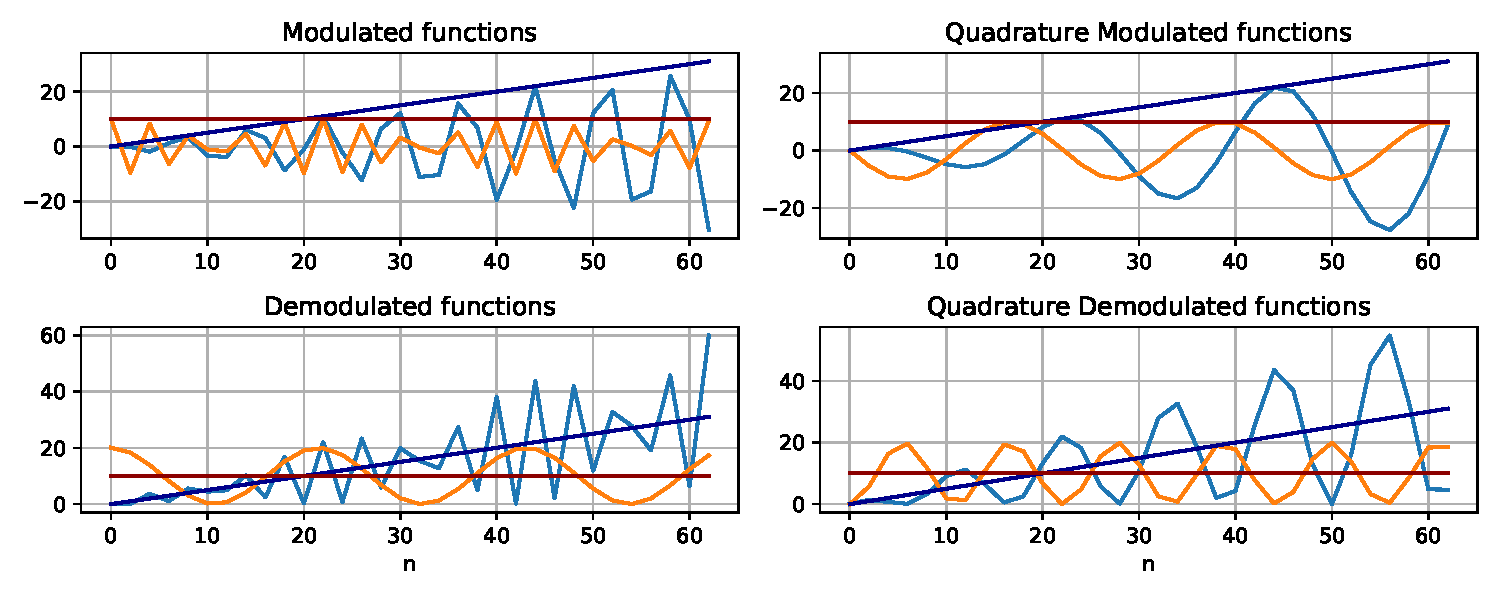
\includegraphics[width=0.9\textwidth]{figures/modulation.pdf}
	\caption{Non-quadrature modulation and demodulation (left). Quadrature modulation and demodulation (right).}
	\label{fig:modulation_visualizations}
\end{figure}

\section{Convolution}

Convolution is implemented in time-domain and as fast convolution using the \ac{FFT}.
To verify the correctness of the implementations,
a sawtooth signal is convolved with a shifted impulse signal.
The results are the same for both implementations within a tolerance smaller than \(\pm10^{-15}\).
When convolving with a shifted impulse signal, the convolution is equal to the shifted signal.
This is shown in Figure \ref{fig:convolution}.
\begin{figure}[h!]
	\centering
	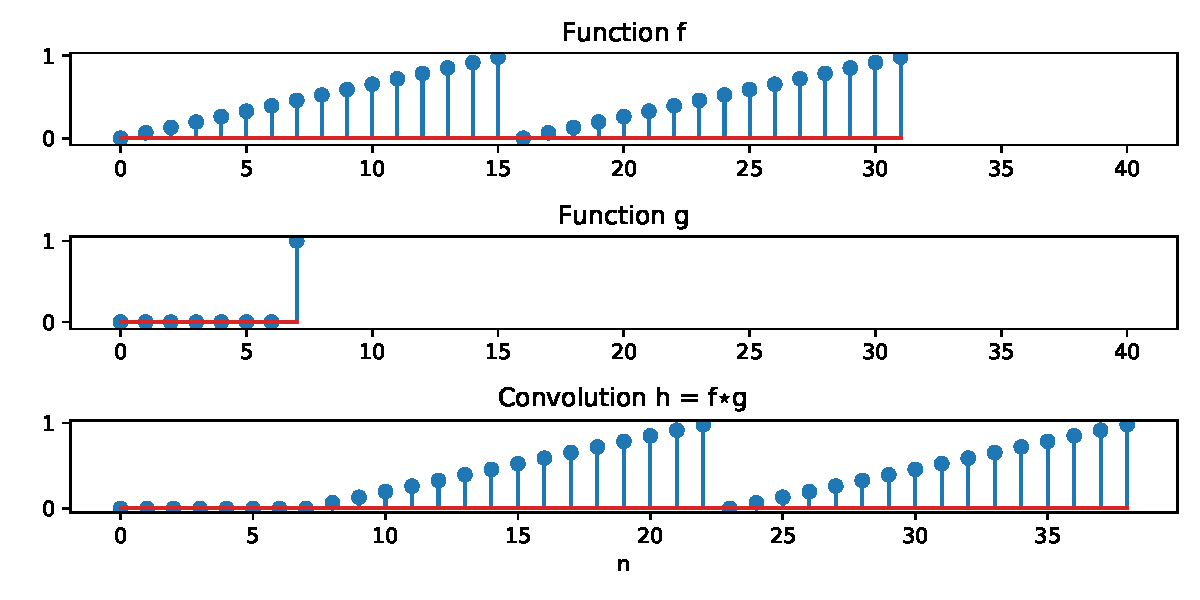
\includegraphics[width=0.7\textwidth]{figures/convolution.pdf}
	\caption{Convolution of a sawtooth signal with a shifted impulse signal.}
	\label{fig:convolution}
\end{figure}

\section{Low-Pass Filter}

The filter is implemented by convolving the input signal with the \(sinc\) function.
By filtering an impulse signal, the filter can be obtained.
Figure \ref{fig:low_pass_filter} (left) shows the filter with and without a Hamming window.

\begin{figure}[h!]
	\centering
	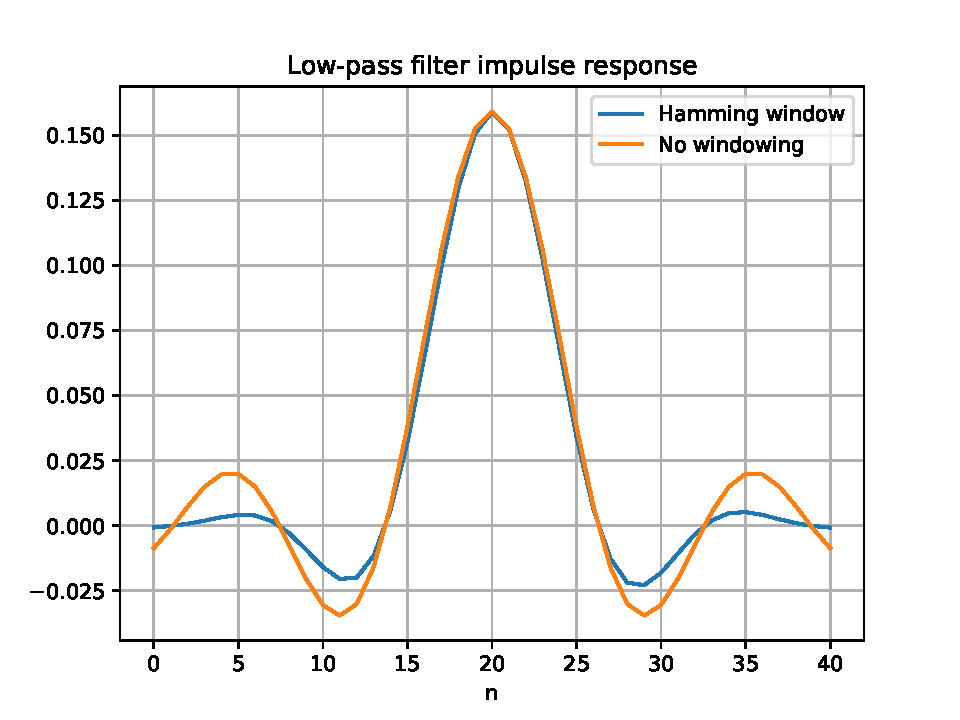
\includegraphics[width=0.4\textwidth]{figures/impulse_response.pdf}
	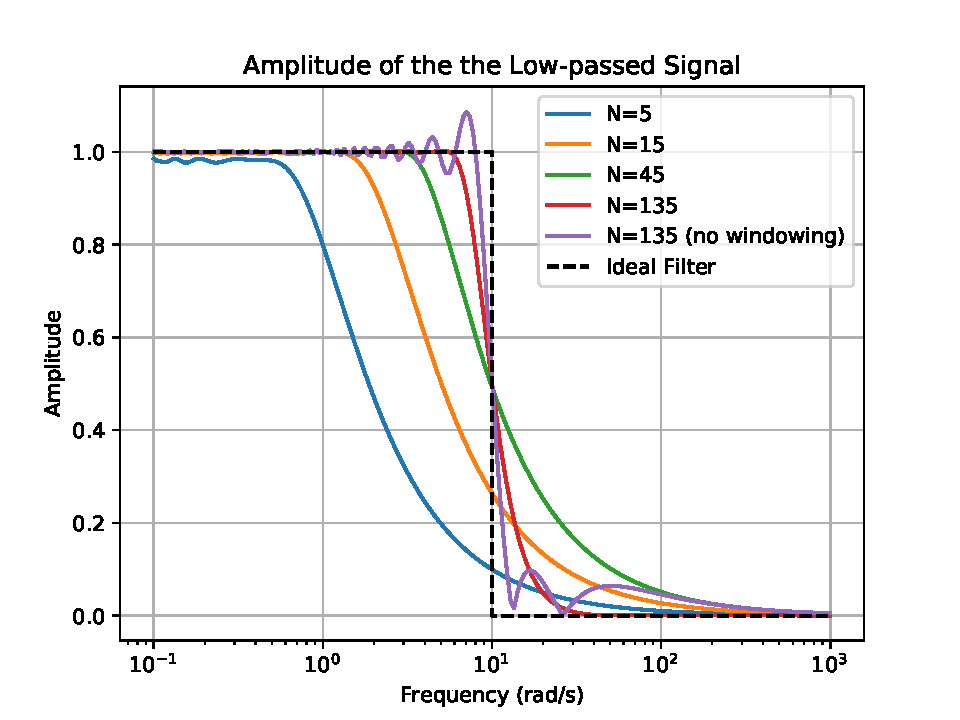
\includegraphics[width=0.4\textwidth]{figures/passband.pdf}
	\caption{Impulse response of the low-pass filter with N=20 (left). Amplitude of the low-passed signal with different filter lengths (right).}
	\label{fig:low_pass_filter}
\end{figure}

The frequency response of the low-pass filter is determined by filtering cosine waves with increasing frequencies
and calculating the highest amplitude of the output signal.
This is shown for different filter lengths in Figure \ref{fig:low_pass_filter} (right).
Here, the cut-off frequency is 10 \({rad}/s\).
It can be observed that the steepness of the transition band increases with the filter length.
If no Hamming window is applied, there are ripples in the passband and the stopband.

The performance of the low-pass filter highly depends on the implementation of the convolution.
Table \ref{tab:timing_comparison} shows the timing comparison when using fast convolution and convolution in time-domain.
For the given parameters, the fast convolution is on average more than 2.4 times faster then in time-domain.
\begin{table}[h!]
	\centering
	\begin{tabular}{|l|c|c|}
		\hline
		                   & \textbf{Fast Convolution} & \textbf{Time-Domain Convolution} \\ \hline
		Average time       & 0.2997 \(s\)              & 0.7241 \(s\)                     \\ \hline
		Standard deviation & 0.0397 \(s\)              & 0.0603 \(s\)                     \\ \hline
		Min time           & 0.2598 \(s\)              & 0.6684 \(s\)                     \\ \hline
		Max time           & 0.5171 \(s\)              & 1.269 \(s\)                      \\ \hline
		Median time        & 0.2864 \(s\)              & 0.715 \(s\)                      \\ \hline
	\end{tabular}
	\caption{Timing comparison for Low-Pass Filter using fast convolution and time-domain convolution. Function length = 20000, Filter length = 50, Number of tests = 200.}
	\label{tab:timing_comparison}
\end{table}

\chapter{Overall system}

The overall system recreates the transmission of two signals over a common medium using modulation.
On the sender side, the signals are low-pass filtered, modulated and added.
The sum of both modulated signals is then transmitted to the receiver,
where the signal is demodulated and low-pass filtered again.

For testing the overall system, the following signals are used.
The first signal is a sum of cosine waves (Equation 1)
and the second signal is a sawtooth wave (Equation 2).
\begin{equation}
	f_1(t) = 3 + cos(t+1) + 2cos(3t+2) - 5cos(4t-1) + cos(13t)
\end{equation}
\begin{equation}
	f_2(t) = 3 \cdot (t\mod\pi)
\end{equation}
Both signals are sampled 32 times in the interval from 0 to 2\(\pi\).
Each step of the transmission is shown in Figure \ref{fig:overall} (top), where the left side depicts the operations in time-domain
and the right side in frequency-domain, by showing the magnitude of the first half of the Fourier coefficients.
The low-pass filtered signals are compared to the reconstructed signals in the bottom figure.

The cut-off frequency is choosen to be \(\omega_c=\) 7 \(rad/s\).
As seen in the second row, the low-pass filter removes the high frequency components.
Furthermore the sampling rate is increased by factor 2 after the low-pass filter,
because modulation would not be possible without violating the sampling theorem.
Then the signals are modulated with \(\omega_{mod_1}=\) 8 \(rad/s\) and \(\omega_{mod_2}=\) 23 \(rad/s\),
so that their frequency bands do not overlap.
After adding, demodulation and low-pass filtering, the reconstructed signals are nearly equal to the original, low-passed signals.

An alternative approach is to use quadrature modulation.
This is shown in Figure \ref{fig:quadrature},
where the signals are modulated with the same modulation frequency \(\omega_{mod}=\) 8 \(rad/s\),
but with a cosine and a sine wave, respectively.

When a overlap of the frequency bands is introduced,
the signals cannot be reconstructed properly.
For this example the signals are sampled 64 times.
The modulation frequencies are \(\omega_{mod_1}=\) 8 \(rad/s\) and \(\omega_{mod_2}=\) 19 \(rad/s\).
This is shown in Figure \ref{fig:overlap},
where the signals contain noise of the other signal.
Most significant is a noise in the sawtooth signal with a frequency of 7 \(rad/s\).


\appendix

\chapter{Figures}

\begin{figure}[h!]
	\centering
	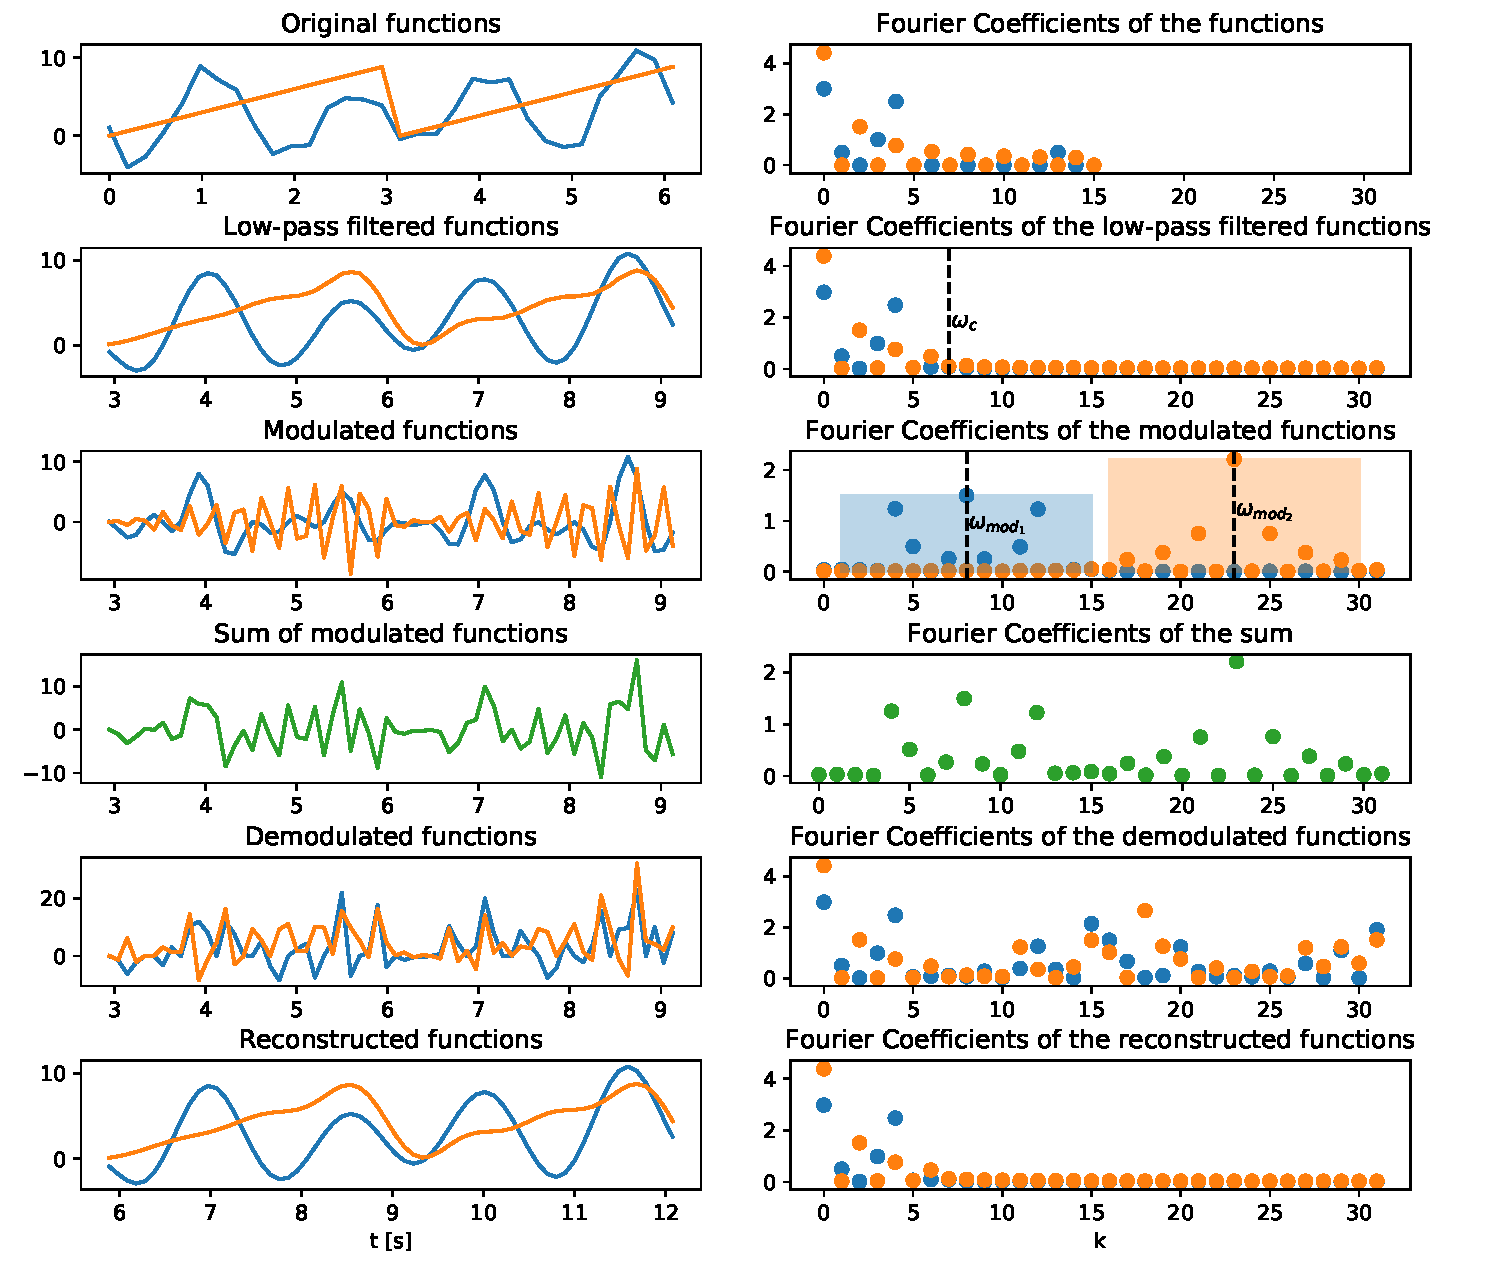
\includegraphics[width=\textwidth]{figures/overall_sampling.pdf}
	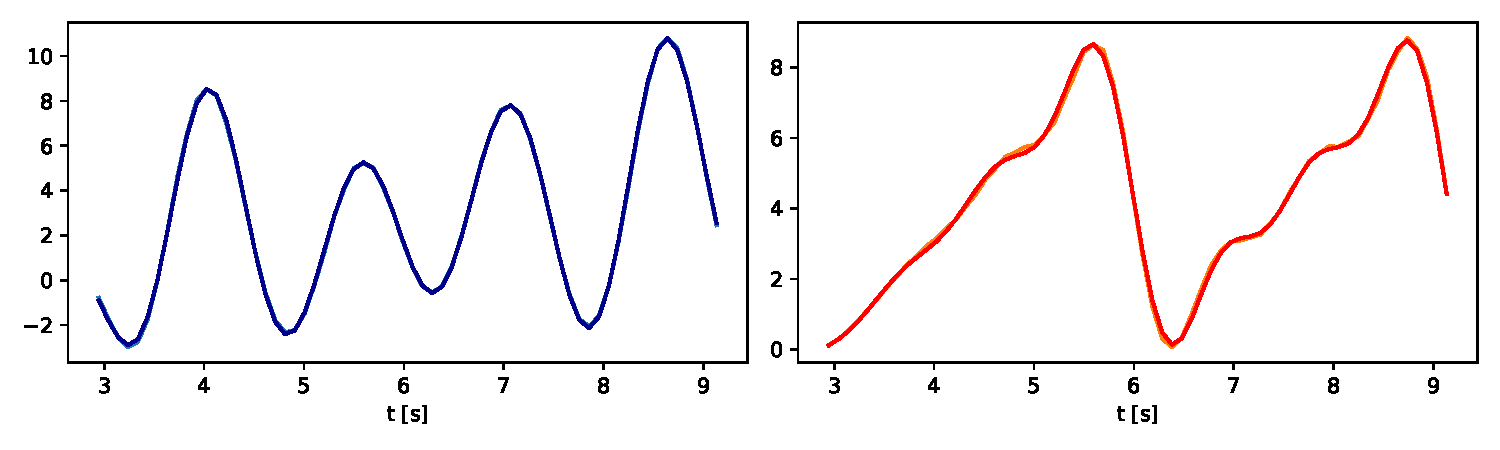
\includegraphics[width=0.9\textwidth]{figures/sampling_cmp.pdf}
	\caption{Overall sytsem (top). Reconstructed vs. low-pass filtered signals (bottom).}
	\label{fig:overall}
\end{figure}


\begin{figure}[h!]
	\centering
	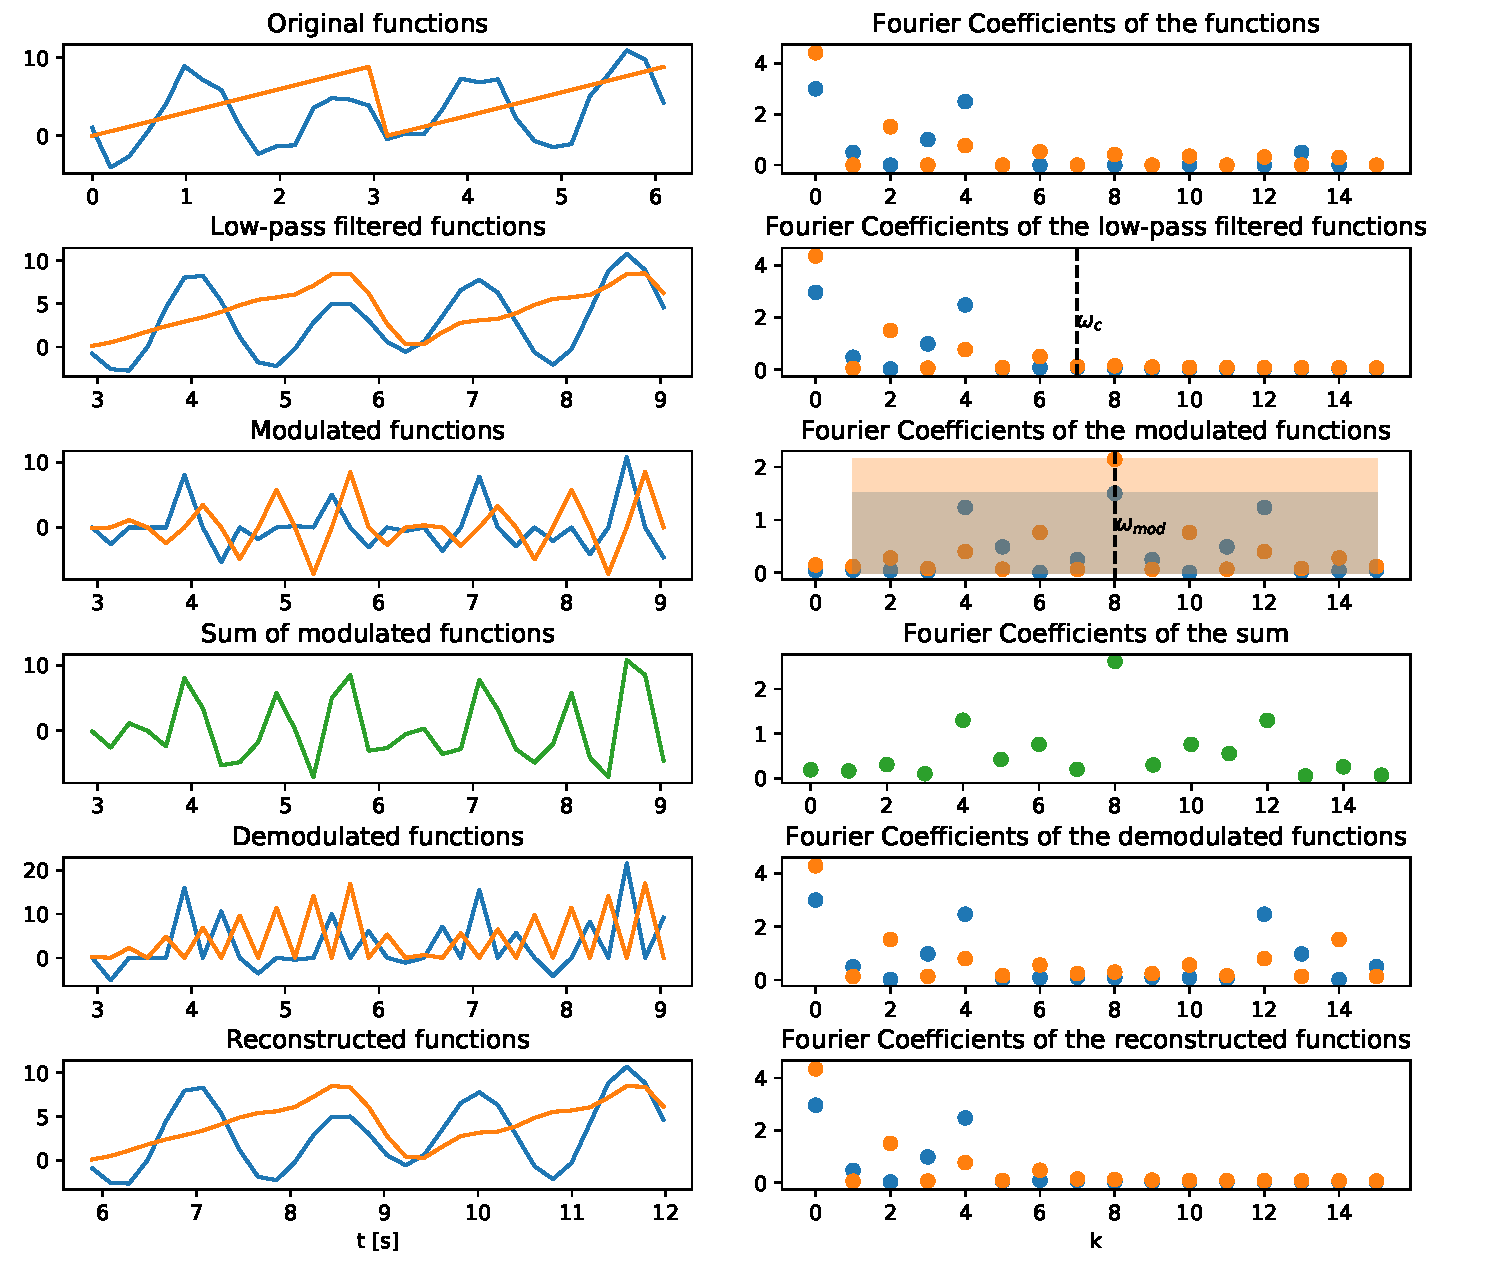
\includegraphics[width=\textwidth]{figures/overall_quad.pdf}
	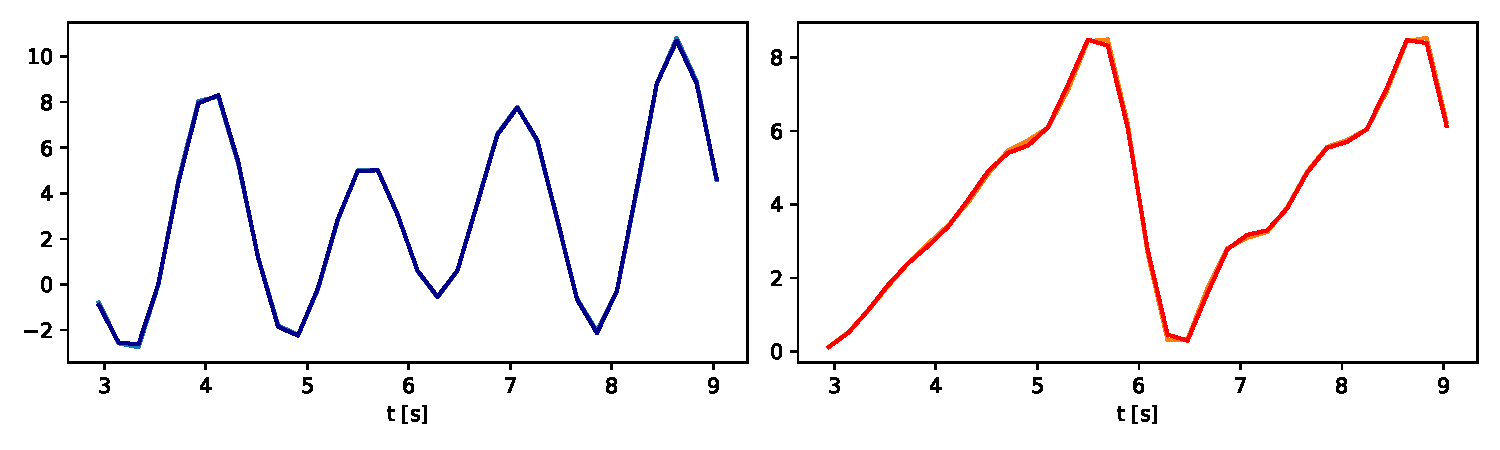
\includegraphics[width=0.9\textwidth]{figures/quad_cmp.pdf}
	\caption{Overall sytsem with quadrature modulation (top). Reconstructed vs. low-pass filtered signals (bottom).}
	\label{fig:quadrature}
\end{figure}

\begin{figure}[h!]
	\centering
	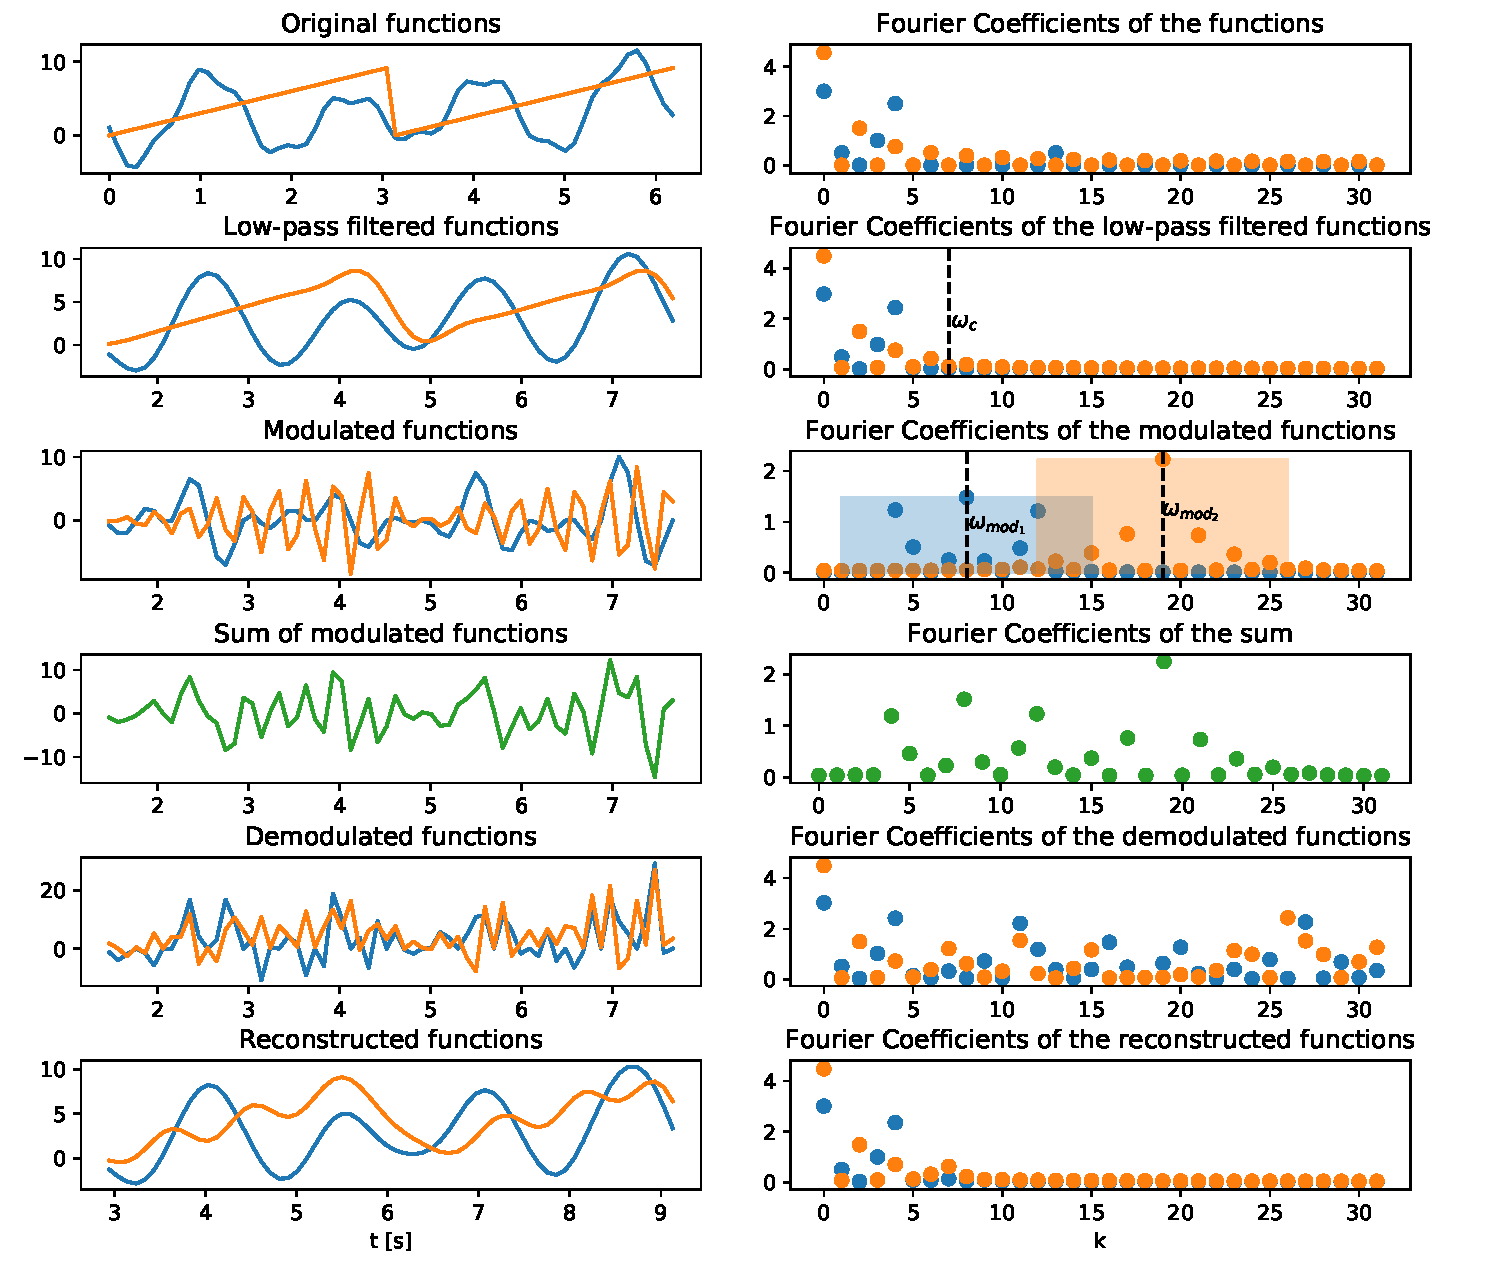
\includegraphics[width=\textwidth]{figures/overall_overlapping.pdf}
	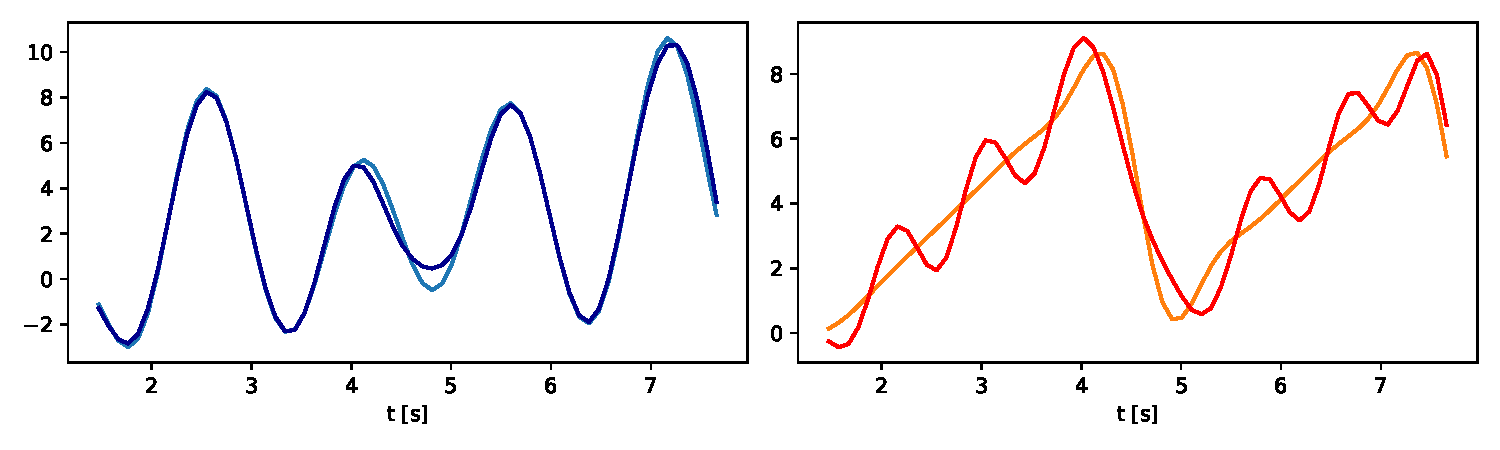
\includegraphics[width=0.9\textwidth]{figures/overlapping_cmp.pdf}
	\caption{Overall sytsem with overlapping frequency bands (top). Reconstructed vs. low-pass filtered signals (bottom).}
	\label{fig:overlap}
\end{figure}

\end{document}
